% SyncFit Edge · 15-minute pitch in the brand style.
% Same script and timing as public/SyncFit-Pitch.html (5 min problem + 10 min live demo).
% Build: cd beamer && xelatex syncfit-pitch.tex  (twice, for the slide count)
% Speaker notes: add "show notes on second screen" to \setbeameroption below.
\documentclass[aspectratio=169,11pt]{beamer}
\usepackage{beamerthemesyncfit}
% \setbeameroption{show notes on second screen=right}

\title{SyncFit Edge}

% Photo with the app's card radius.
\newcommand{\foto}[3]{% {file}{width}{height}
  \begin{tikzpicture}
    \clip[rounded corners=16pt] (0,0) rectangle (#2,#3);
    \node[anchor=south west, inner sep=0pt] at (0,0) {\includegraphics[width=#2,height=#3,keepaspectratio=false]{#1}};
  \end{tikzpicture}}
\newcommand{\titular}[1]{{\display\fontsize{26}{27}\selectfont #1\par}}

\begin{document}

% ---------------------------------------------------------------- 1
\begin{frame}[plain]
  \begin{tikzpicture}[remember picture, overlay]
    \nube{$(current page.north west)+(-1,-1.6)$}{3.6}
    \nube[nube!70!rosa]{$(current page.south east)+(-4.2,1.4)$}{3}
    \nube[rosaclaro]{$(current page.north east)+(-3.4,-.9)$}{1.8}
  \end{tikzpicture}
  \vspace{.4cm}
  \begin{columns}[c]
    \column{.5\textwidth}
      \minutos{00:00 – 02:00}\par\vspace{.5cm}
      \titular{El contexto cambia. La rutina también.}
      \vspace{.4cm}
      {\normalsize Una atleta llega al gimnasio con menos energía y encuentra que su máquina habitual está ocupada. ¿Cómo decide qué entrenar hoy?\par}
    \column{.44\textwidth}
      \foto{img/athlete.jpg}{6cm}{4.5cm}
  \end{columns}
  \begin{tikzpicture}[remember picture, overlay]
    \node[anchor=south west, inner sep=0pt] at ($(current page.south west)+(.6,.4)$)
      {
\includegraphics[height=.42cm]{img/pulsi.png}\hspace{4pt}{\display\color{ink}\normalsize syncfit}};
    \node[anchor=south east, font=\footnotesize\bfseries, text=inksuave] at ($(current page.south east)+(-.6,.45)$)
      {El problema \textperiodcentered\ 1 de 6};
  \end{tikzpicture}
  \note{Abre con la escena: misma atleta, otro día, otro cuerpo. Deja la pregunta en el aire antes de pasar.}
\end{frame}

% ---------------------------------------------------------------- 2
{\setbeamercolor{background canvas}{bg=lavanda}\setbeamercolor{normal text}{fg=lavandatexto}
\setbeamertemplate{footline}{%
  \begin{tikzpicture}[remember picture, overlay]
    \node[anchor=south east, font=\footnotesize\bfseries, text=lavandatexto] at ($(current page.south east)+(-.6,.45)$)
      {El problema \textperiodcentered\ 2 de 6};
  \end{tikzpicture}}
\begin{frame}
  \begin{tikzpicture}[remember picture, overlay]
    \gotea{rosa}{.75}
  \end{tikzpicture}
  \vspace{.35cm}
  \tikz\node[fill=lavandanoche, text=lavandatexto, rounded corners=7pt, inner xsep=8pt, inner ysep=3pt, font=\small\bfseries]{02:00 – 05:00};\par\vspace{.3cm}
  {\color{nube}\titular{¿Qué cambia hoy?}}
  \vspace{.05cm}
  {\small\color{lavandatexto} Pregunta al público qué información usaría para ajustar la rutina. Elige una respuesta para mostrar cómo entra al flujo de SyncFit.\par}
  \vspace{.1cm}
  \color{ink}
  \onslide<1->{\tarjeta{menstrualsuave}{3.75cm}{Ciclo o gestación}{\textbf{Contexto fisiológico.} La fase del ciclo o la etapa de gestación aporta contexto al generar una propuesta de entrenamiento.}}\hfill
  \onslide<2->{\tarjeta{folicularsuave}{3.75cm}{Energía}{\textbf{Energía percibida.} La atleta registra cómo se siente. SyncFit usa esa información junto con las señales de la captura para ajustar la propuesta.}}\hfill
  \onslide<3->{\tarjeta{ovulatoriasuave}{3.75cm}{Equipo}{\textbf{Inventario del gimnasio.} El plan puede priorizar ejercicios asociados a las máquinas que están registradas en el gimnasio activo.}}
  \note{Pide respuestas al público. Revela una tarjeta por respuesta: ciclo, energía, equipo. Son las tres entradas de la rutina.}
\end{frame}}

% ---------------------------------------------------------------- 3
\renewcommand{\parte}{Demostración}
\begin{frame}
  \begin{tikzpicture}[remember picture, overlay]
    \nube[rosaclaro]{$(current page.north east)+(-4.6,-1.2)$}{3.4}
  \end{tikzpicture}
  \minutos{05:00 – 06:00}\par\vspace{.3cm}
  \titular{Dos accesos, dos tareas}
  \vspace{.2cm}
  {\normalsize Abre el entorno de evaluación en dos perfiles del navegador. Usa los accesos rápidos existentes.\par}
  \vspace{.5cm}
  \tarjeta{nube}{3.75cm}{Administrador de gimnasio}{Abre el panel y elige el gimnasio de prueba.}\hfill
  \tarjeta{nube}{3.75cm}{Atleta}{Abre la app y prepara el código para unirte al gimnasio de prueba.}\hfill
  \tarjeta{nube}{3.75cm}{Superadministrador}{Ten abierta la sesión de catálogos para el ejercicio del minuto nueve.}
  \note{Deja las tres sesiones listas antes de empezar: gimnasio, atleta y super admin.}
\end{frame}

% ---------------------------------------------------------------- 4
\begin{frame}
  \begin{tikzpicture}[remember picture, overlay]
    \nube{$(current page.south west)+(-1,1.2)$}{3.2}
  \end{tikzpicture}
  \begin{columns}[c]
    \column{.48\textwidth}
      \minutos{06:00 – 09:00}\par\vspace{.4cm}
      \titular{Registra una máquina}
      \vspace{.4cm}
      {\normalsize En el panel del gimnasio, crea una máquina y vincúlala con un ejercicio. Al recargar, el inventario y el contador reflejan el cambio guardado.\par}
    \column{.46\textwidth}
      \foto{img/machine.jpg}{6cm}{4.5cm}\par
      {\footnotesize\color{inksuave} Máquina ilustrativa.}
  \end{columns}
  \note{Panel del gimnasio: nueva máquina, foto, ejercicio vinculado. Recarga para mostrar que se guardó.}
\end{frame}

% ---------------------------------------------------------------- 5
\begin{frame}
  \minutos{09:00 – 11:00}\par\vspace{.3cm}
  \titular{Agrega un grupo muscular}
  \vspace{.2cm}
  {\normalsize Explora cómo una opción de Superadministración llega a la rutina de la atleta.\par}
  \vspace{.1cm}
  \begin{tikzpicture}[x=1cm, y=1cm]
    \fill[nube, rounded corners=3pt] (0,1.95) rectangle (13.6,2.15);
    \only<1>{\fill[ink, rounded corners=3pt] (0,1.95) rectangle (2.2,2.15);}
    \only<2>{\fill[ink, rounded corners=3pt] (0,1.95) rectangle (6.7,2.15);}
    \only<3>{\fill[ink, rounded corners=3pt] (0,1.95) rectangle (13.6,2.15);}
    \foreach \x/\n/\c/\t/\d [count=\i] in {
      0/1/luteasuave/Crea el grupo/En Catálogos $\rightarrow$ Opciones{,} crea un grupo muscular de prueba.,
      4.75/2/folicularsuave/Asocia un ejercicio/En Ejercicios{,} añade el identificador del grupo al campo muscle\_groups del ejercicio.,
      9.5/3/ovulatoriasuave/Comprueba la rutina/Desde la sesión de atleta{,} recarga la vista de rutina y selecciona el grupo nuevo.} {
      \node[fill=\c, rounded corners=14pt, text width=3.9cm, inner sep=7pt, anchor=north west, align=left, opacity=1] at (\x,1.6)
        {{\scriptsize\bfseries 0\n}\par{\display\normalsize \t}\par\vspace{2pt}{\scriptsize\hyphenpenalty=10000 \d}};
    }
    \only<1>{\node at (2.2,2.4) {
\includegraphics[height=1cm]{img/pulsi.png}};}
    \only<2>{\node at (6.7,2.4) {
\includegraphics[height=1cm]{img/pulsi.png}};}
    \only<3>{\node at (13.1,2.4) {
\includegraphics[height=1cm]{img/pulsi.png}};}
  \end{tikzpicture}
  \note{Avanza por los tres pasos; Pulsi recorre la línea como en la landing. Cierra mostrando el grupo nuevo en la rutina.}
\end{frame}

% ---------------------------------------------------------------- 6
{\setbeamercolor{background canvas}{bg=ovulatoriasuave}
\begin{frame}
  \begin{tikzpicture}[remember picture, overlay]
    \nube{$(current page.north west)+(-.8,-1.4)$}{3}
    \nube[nube!80!ovulatoriasuave]{$(current page.south east)+(-3.6,1.1)$}{2.6}
  \end{tikzpicture}
  \begin{columns}[c]
    \column{.5\textwidth}
      \minutos{11:00 – 15:00}\par\vspace{.4cm}
      \titular{Genera la rutina}
      \vspace{.4cm}
      {\normalsize Activa el gimnasio de prueba, elige el grupo muscular y registra tu energía. Genera la rutina con telemetría simulada y revisa qué ejercicios, carga y equipo propone SyncFit.\par}
    \column{.44\textwidth}
      \foto{img/training.jpg}{6cm}{4.5cm}\par
      {\footnotesize\color{inksuave} Ejercicio ilustrativo.}
  \end{columns}
  \note{Atleta: activa el gimnasio, grupo muscular, energía, generar. Comenta ejercicios, carga (k\_load) y equipo propuesto.}
\end{frame}}

\end{document}
